\documentclass[11pt]{article}
\usepackage[letterpaper,margin=0.72in,headheight=15pt]{geometry}
\usepackage{amssymb,array,booktabs,fancyhdr,graphicx,listings,microtype,tabularx,tikz,xcolor}
\usepackage[hidelinks]{hyperref}
\hypersetup{pdftitle={ADK Lesson 018: Inert access-control trainer},
pdfauthor={Kevin Shanahan},pdfsubject={Deterministic keypad entry, lockout, fault handling, and inert output intent},pdflang={en-US}}
\usetikzlibrary{arrows.meta,positioning}
\graphicspath{{docs/lessons/assets/}{../assets/}}
\definecolor{soft}{gray}{0.94}\definecolor{mid}{gray}{0.45}
\definecolor{codebg}{gray}{0.97}
\pagestyle{fancy}\fancyhf{}\lhead{\textsc{ADK field lesson 018}}
\rhead{Inert access trainer}\cfoot{\thepage}
\setlength{\parindent}{0pt}\setlength{\parskip}{5pt}
\renewcommand{\arraystretch}{1.18}
\lstdefinestyle{adkcpp}{language=C++,basicstyle=\ttfamily\small,
backgroundcolor=\color{codebg},frame=single,rulecolor=\color{mid},
columns=fullflexible,keepspaces=true,showstringspaces=false,breaklines=true}
\newcommand{\checkbox}{\(\square\)}
\newcommand{\blankline}{\rule{0.96\linewidth}{0.35pt}}
\begin{document}

\begin{center}
{\Huge\bfseries Separate intent from physical truth}\\[3pt]
{\Large Lesson 018: inert access-control trainer}\\[6pt]
\textit{Observe $\rightarrow$ decide $\rightarrow$ present $\rightarrow$ replay}
\end{center}
\begin{center}
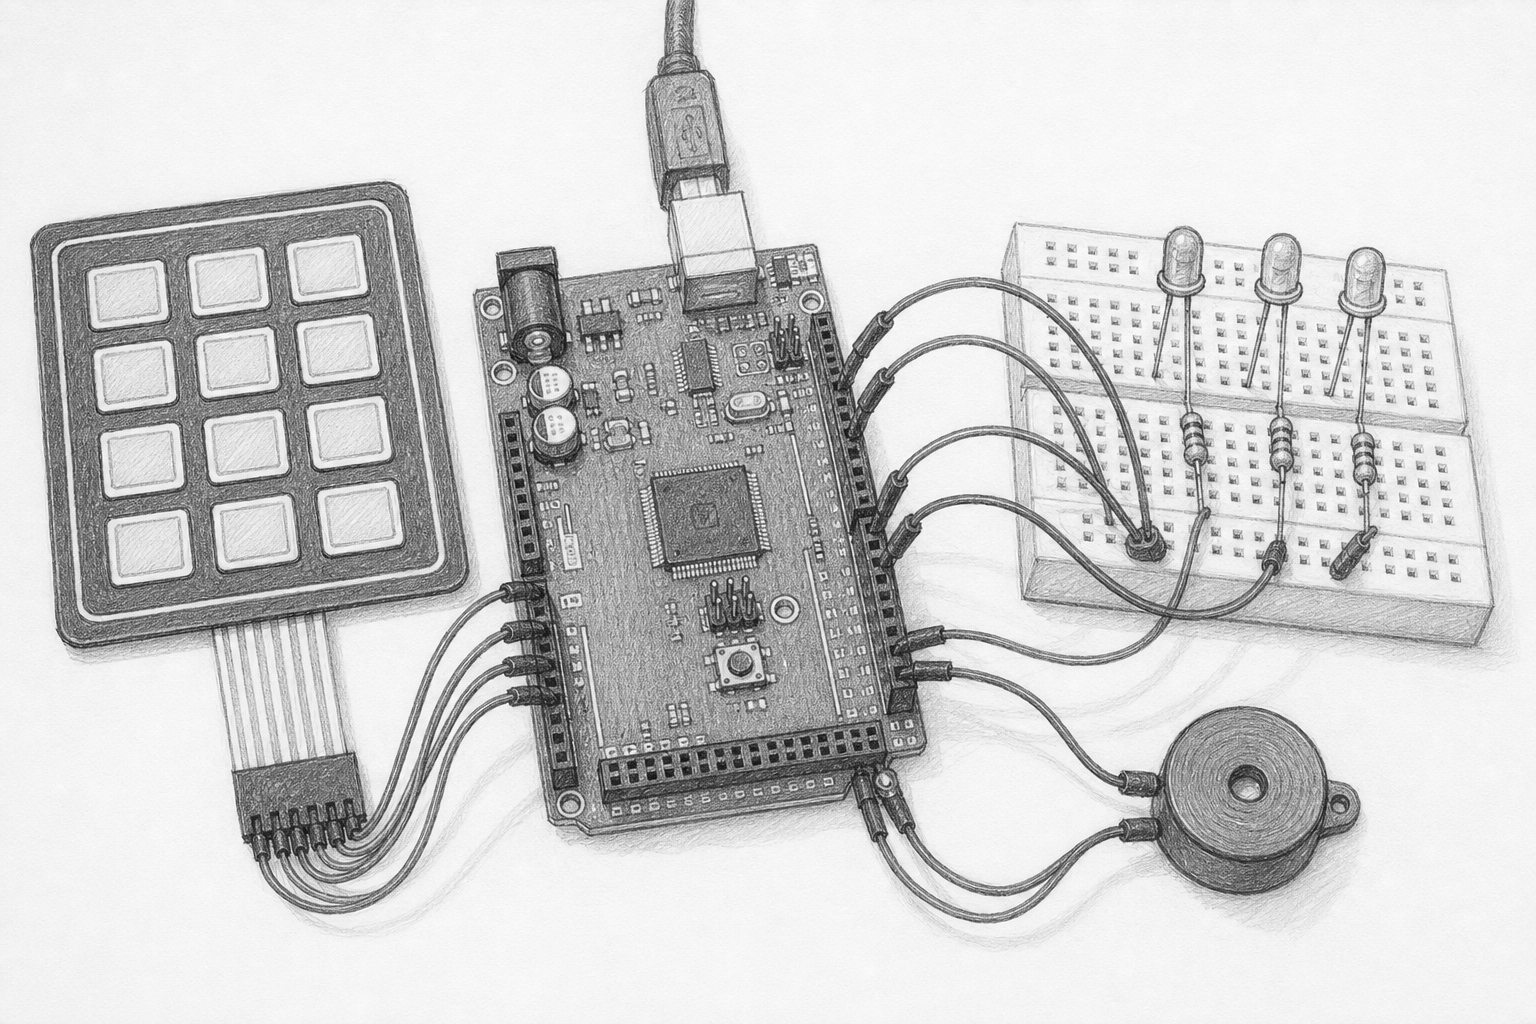
\includegraphics[width=\linewidth,height=0.28\textheight,keepaspectratio]
{018-access-trainer-pencil.png}
\end{center}
\textbf{Orientation plate.} The pencil drawing helps identify the Mega, keypad,
three status channels, and optional sounder. It is not a wiring diagram. This
first E1 build omits the sounder; the net table below is authoritative.

\begin{tabularx}{\linewidth}{@{}>{\bfseries}lX@{}}
Question & Can an input policy remain deterministic, observable, and inert
through grants, denials, lockout, faults, reset, and shutdown?\\
Time & 100--140 minutes\\
Prerequisites & Lessons 010, 014, 016, and the host-only Lesson 017 model\\
You need & Mega 2560, USB, 4×3 passive matrix keypad, common-cathode RGB LED,
four resistors of at least 220\,\(\Omega\), 16×2 HD44780 module, breadboard,
jumpers, multimeter or logic analyzer\\
Evidence & TP-R0 scan, D13 acquisition, RGB state, display prompt/count,
D30 soft-latch intent, shutdown pin state, deterministic audit trace\\
Safety class & E1: logic and low-current indicators only; no motion or load
supply\\
Status & Host verified; physical acceptance open; not a security component\\
\end{tabularx}

\section*{Safety and meaning boundary}

This is a tabletop state-machine trainer. It does not control a lock, door,
cabinet, alarm, relay, solenoid, motor, servo, radio, valuable property, or
real credential. ``Granted'' is a software state. D30 means only
\textbf{open requested}; it never proves a physical thing is open.

Remove USB before wiring. Identify the keypad pinout by its manufacturer data
or unpowered continuity measurements. Give every LED its own resistor. Follow
the identified LCD module's contrast and backlight ratings. Stop for heat,
odor, smoke, USB resets, an unknown module, or a voltage outside 0--5\,V.

\section*{1. Build two independent evidence paths}

\begin{center}
\begin{tabularx}{0.96\linewidth}{@{}lllX@{}}
\toprule
Role & Mega pins & Observation & Meaning\\\midrule
keypad rows & D22--D25 & TP-R0 at D22 & scan activity only\\
keypad columns & D26--D28 & interpreted event & bounded operator input\\
RGB channels & D5/D6/D7 & state color & redundant state presentation\\
soft-latch LED & D30 & off/on & closed/open software intent only\\
acquisition LED & D13 built-in & off/on & all owners acquired\\
LCD & D34--D39 & prompt/count & state without credential digits\\
\bottomrule
\end{tabularx}
\end{center}

\begin{center}
\begin{tikzpicture}[>=Latex,node distance=7mm,
box/.style={draw,rounded corners,fill=soft,text width=27mm,
minimum height=11mm,align=center}]
\node[box] (keys) {4×3 keypad\\TP-R0};
\node[box,right=of keys] (matrix) {\texttt{MatrixKeypad}\\debounced event};
\node[box,right=of matrix] (engine) {\texttt{AccessTrainer}\\pure policy};
\node[box,right=of engine,yshift=15mm] (rgb) {RGB + LCD\\state evidence};
\node[box,right=of engine,yshift=-15mm] (intent) {D30 LED\\soft-latch intent};
\draw[->,thick] (keys)--(matrix);\draw[->,thick] (matrix)--(engine);
\draw[->,thick] (engine)--(rgb);\draw[->,thick] (engine)--(intent);
\end{tikzpicture}
\end{center}

D13 is deliberately outside this chain: it proves acquisition separately.
RGB is not sole evidence because color may be confused or a channel may fail.
The display never echoes entered digits. Serial may record audit intent, but
it cannot replace any circuit observation.

\section*{2. Read the state policy}

\begin{center}
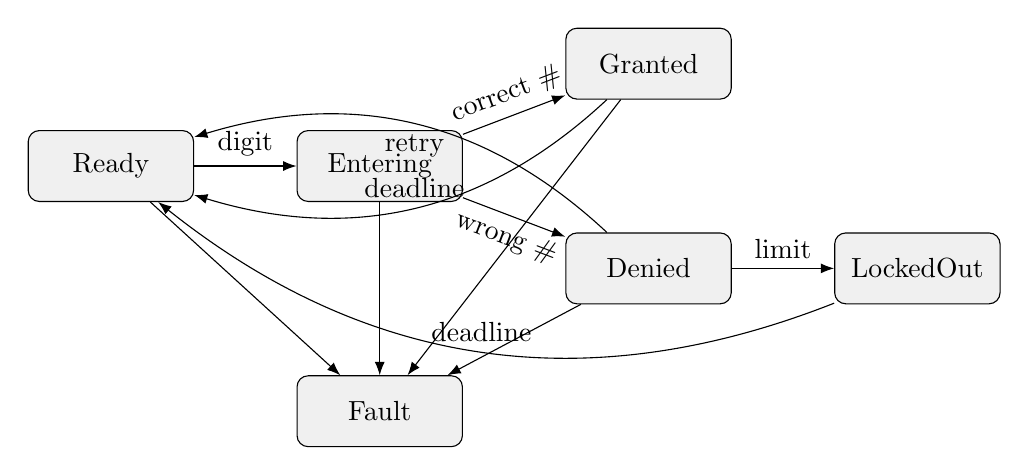
\begin{tikzpicture}[>=Latex,node distance=13mm,
state/.style={draw,rounded corners,fill=soft,minimum width=21mm,
minimum height=9mm,align=center}]
\node[state] (ready) {Ready};
\node[state,right=of ready] (enter) {Entering};
\node[state,right=of enter,yshift=13mm] (grant) {Granted};
\node[state,right=of enter,yshift=-13mm] (deny) {Denied};
\node[state,right=of deny] (lock) {LockedOut};
\node[state,below=22mm of enter] (fault) {Fault};
\draw[->] (ready)--node[above]{digit}(enter);
\draw[->] (enter)--node[above,sloped]{correct \#}(grant);
\draw[->] (enter)--node[below,sloped]{wrong \#}(deny);
\draw[->] (grant) to[bend left] node[above]{deadline}(ready);
\draw[->] (deny) to[bend right] node[below]{retry}(ready);
\draw[->] (deny)--node[above]{limit}(lock);
\draw[->] (lock) to[bend left] node[above]{deadline}(ready);
\draw[->] (ready)--(fault);\draw[->] (enter)--(fault);
\draw[->] (grant)--(fault);\draw[->] (deny)--(fault);
\end{tikzpicture}
\end{center}

Digits append to a bounded teaching entry. \texttt{Star} clears.
\texttt{Hash} submits. Wrong length and wrong value have the same public
behavior. Three failures enter timed lockout. A keypad fault, component fault,
clock rollback, or internal failure enters \texttt{Fault}, requests closed
intent, and requires explicit reset after the fault clears.

\begin{tabularx}{\linewidth}{@{}lXXX@{}}
\toprule
State & RGB & Display & D30\\\midrule
Ready & blue & READY & off\\
Entering & white & ENTER + count & off\\
Granted & green & GRANTED & on\\
Denied & amber & DENIED & off\\
LockedOut & slow amber pulse & LOCKED OUT & off\\
Fault & red & FAULT & off\\
\bottomrule
\end{tabularx}

\section*{3. Keep the engine pure}

\texttt{AccessTrainer} owns no pin, timer, display, storage, callback, or
clock. The application supplies \texttt{TimePoint} and a
\texttt{KeypadSnapshot}; the resulting \texttt{AccessSnapshot} publishes state,
status, LED intent, soft-latch intent, counts, and one audit intent. The typed
intent is \texttt{SoftLatchIntent}. The example consumes each audit intent
immediately into a fixed one-record display sink: row two shows its four-digit
presentation sequence and kind for one second, then returns to entry count.
There is no hidden audit history, allocation, credential copy, or callback.

\begin{lstlisting}[style=adkcpp]
const adk::TimePoint now (millis ());

const adk::KeypadSnapshot operatorInput = observeOperator (now);
const adk::AccessSnapshot decision      = decideAccess    (
    now, operatorInput);

if (!presentAccess (decision))
{
    enterVisibleFault (now);
}
\end{lstlisting}

The emerging Lesson 017 types can translate a future \texttt{SoftLatchIntent} into
a bounded position. This lesson instead translates \texttt{softLatchOpen} to
D30. That adapter choice preserves the high-level story while keeping hardware
inert.

\section*{4. Predict exact traces}

Use a fixed four-key teaching fixture. Do not use a real PIN or reuse any
credential. For every row, predict state, entered count, failed attempts,
D30, and whether one audit intent appears.

\begin{tabularx}{\linewidth}{@{}lXXXXX@{}}
\toprule
Input/time & State & Count & Failures & D30 & Audit\\\midrule
boot/reset & & & & &\\
first digit & & & & &\\
\texttt{Star} & & & & &\\
correct + \texttt{Hash} & & & & &\\
grant deadline $-1$ & & & & &\\
grant deadline & & & & &\\
wrong submit ×3 & & & & &\\
lockout deadline $-1$ & & & & &\\
lockout deadline & & & & &\\
keypad fault & & & & &\\
\bottomrule
\end{tabularx}

\textbf{Rollover exercise.} Start a grant immediately before
\texttt{uint32\_t} time wraps. Supply the same elapsed intervals on two runs.
Snapshots and audit records must match byte for byte.

\section*{5. Test failures before the breadboard}

\begin{enumerate}
\item empty, one-key, maximum-length, extra-key, clear, and submit paths;
\item wrong length and wrong value with indistinguishable public timing;
\item failure threshold and lockout one tick before, at, and after deadline;
\item chord/stuck behavior without appended digits;
\item keypad and component faults from every active state;
\item time rollback and timestamp wrap;
\item audit capacity without hidden allocation or entered digits;
\item reset and shutdown from every state, always with closed intent;
\item two identical traces with identical snapshots and audit records;
\item hardware claim failure and rollback for keypad, RGB, LCD, D30, and D13.
\end{enumerate}

\begin{lstlisting}[style=adkcpp]
make host-test-access-trainer
make quality-fast
make arduino-Lesson018AccessTrainer
\end{lstlisting}

Host evidence establishes policy, not security or physical acceptance.

\section*{6. Run the circuit-native experiment}

\begin{lstlisting}[style=adkcpp]
make boards
make arduino-Lesson018AccessTrainer
make upload EXAMPLE=Lesson018AccessTrainer PORT=/dev/ttyACM0
make hardware-card LESSON=018
make monitor PORT=/dev/ttyACM0 BAUD=115200
\end{lstlisting}

\begin{enumerate}
\item With USB removed, continuity-check keypad identity, LED resistors, common
ground, and absence of every actuator/load connection.
\item Apply USB. D13 should turn on only after all resources initialize.
\item Probe TP-R0 and press one key. Interpret scan activity separately from
the accepted entry shown by RGB/LCD.
\item Replay correct, denied, lockout, clear, invalid chord, and fault traces.
Confirm each audit event appears briefly as \texttt{A\#\#\#\# KIND} before row two
returns to entry count.
\item During lockout, confirm the amber RGB state alternates 500\,ms on and
500\,ms off while the LCD remains \texttt{LOCKED OUT}.
\item At every non-granted state, verify D30 is off. During granted, say
``open requested,'' not ``open.''
\item Invoke the published shutdown path. Verify indicators inactive, then use
an instrument to check released pins rather than inferring from darkness.
\end{enumerate}

\begin{tabularx}{\linewidth}{@{}p{0.22\linewidth}p{0.30\linewidth}X@{}}
\toprule
Observation & Next check & Interpretation\\\midrule
D13 off & initialization status and claims & acquisition failed; no state claim\\
TP-R0 active, no entry & keypad column identity and snapshot & scan exists;
event may not\\
state changes, D30 fixed & probe D30 before LED resistor & separates command
from load wiring\\
D30 on outside grant & remove USB immediately; inspect adapter & policy/presentation
contract violated\\
RGB and LCD disagree & enter fault and close intent & presentation evidence is
contradictory\\
Serial disagrees & trust neither; replay host trace and circuit evidence &
text is supporting evidence only\\
\bottomrule
\end{tabularx}

\section*{7. Explain the deferred motion gate}

\texttt{ServoOutput} construction is inert and owns its signal pin and timer
transactionally. \texttt{BoundedServo} rejects positions outside validated
calibration. Those software properties do not make motion accepted.

Do not add a servo to this circuit. A later E2 variant first requires Lesson
017 physical acceptance with an identified servo, external current-limited
supply, physical switch in servo-positive, common-ground review, D44/Timer5
waveform evidence, restrained paper pointer, current measurements, motion
envelope, and an independent load-power stop. No door, lock, linkage, relay,
solenoid, or useful load is admitted. A destructor is not a stop switch.

\section*{Acceptance record}

\begin{tabularx}{\linewidth}{@{}>{\bfseries}lX@{}}
Board, USB supply, date &\\
Keypad identity / unpowered map &\\
LED and LCD ratings/resistors &\\
D13 acquisition observation &\\
TP-R0 observation &\\
Ready/Entering/Granted/Denied/LockedOut/Fault evidence &\\
D30 closed/open-intent evidence &\\
Reset and shutdown pin evidence &\\
Host replay and audit result &\\
Deviations and reviewer &\\
\end{tabularx}

\checkbox\ no actuator or load supply \quad
\checkbox\ no real credential \quad
\checkbox\ acquisition and output evidence separate \quad
\checkbox\ physical acceptance recorded, not inferred

\vfill\small
\textbf{Companion material.} HTML carries current API signatures, source
links, errata, and searchable CLI procedures. This PDF carries predictions,
state traces, diagnosis, and bench sign-off. The orientation drawing was
generated with the built-in image tool; the schematic and net table govern.

\href{https://docs.arduino.cc/hardware/mega-2560/}{Arduino Mega 2560}\quad
\href{https://www.microchip.com/en-us/product/ATmega2560}{ATmega2560}
\end{document}
